\chapter{Human gait pattern}
\label{Human gait pattern}
\hfill \break

The gait pattern, also known as the gait cycle, refers to the sequence of movements that occur when a person walks or runs. The process of dividing the gait cycle into specific phases has been widely accepted by experts in the field. Jacquelin Perry, in 1992 \cite{Perry:1992}, proposed a functional division of the gait cycle into eight phases, which is based on biomechanical function and neuromuscular activity. This division is not based on equal time intervals but on distinct units of different duration. The assignment of a step phase always refers to a specific leg, while the contralateral leg is simultaneously in a corresponding phase. Perry's work was later modified by Sutherland et al. (1988) and Winter (1990), and these modifications have also been widely accepted by experts in the field. Ultimately, the crucial factor in determining the appropriate division of the gait cycle is the functional perspective under which the gait pattern is to be analyzed. \cite{Ludwig:2022}
\section{Phases of the gait cycle}
The gait cycle, as proposed by Jacquelin Perry in 1992 \cite{Perry:1992}  , is a framework for understanding the sequence of events that occur during the act of walking. The cycle is divided into eight distinct phases, each of which is characterized by specific biomechanical functions and neuromuscular activity. These phases are not based on equal time intervals, but rather on distinct units of varying duration. \ref{Images/GCycle}
\begin{figure}
	\centering
	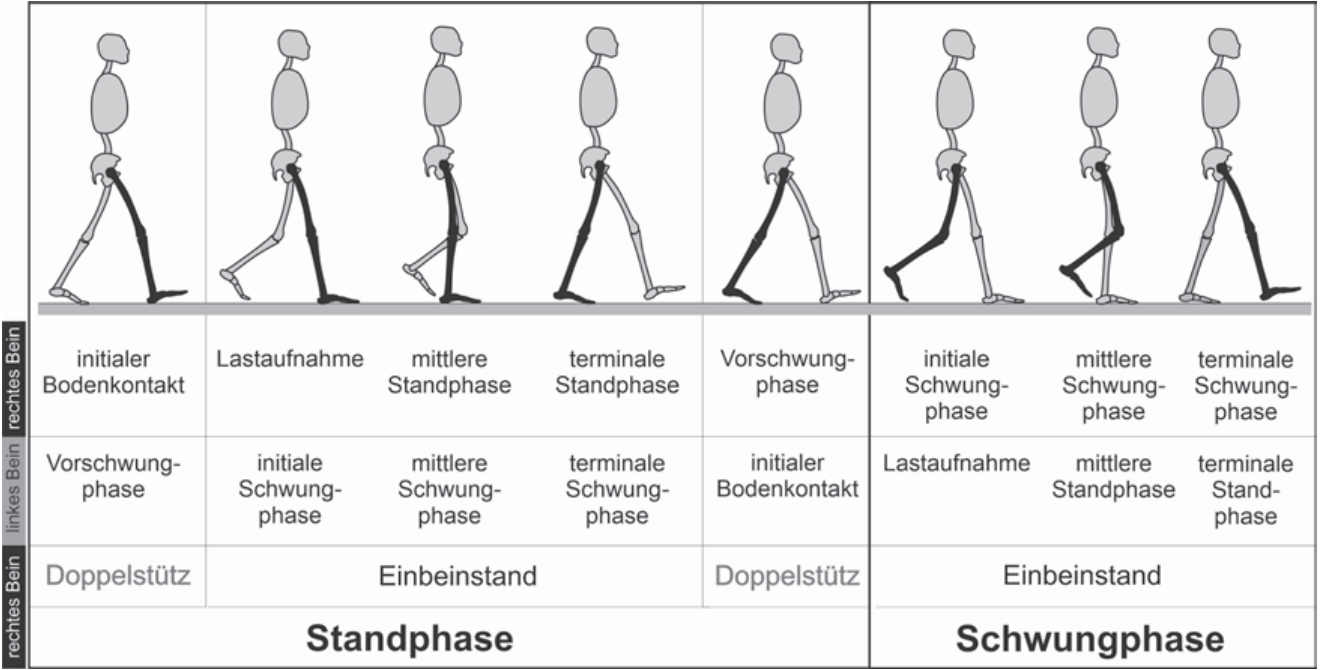
\includegraphics[width=1\textwidth]{Images/GCycle}
	\caption{Schematic representation of the gait cycle \cite{Ludwig:2022} }
\end{figure}


The first phase, Initial Contact, marks the beginning of the gait cycle as the foot touches the ground, typically in the lateral heel area. This phase poses a neurobiomechanical challenge as the lower limb must be stabilized to bear the body weight and simultaneously cushion the impact of landing, making the motion smooth and efficient.

The second phase, Loading Response, marks the transfer of body weight from the rear leg to the front leg, and the slight shift of the center of gravity to the side of the front leg. The rear leg begins to lift off the ground.

The third phase, Midstance, is characterized by the body weight being supported by one leg and the knee of the supporting leg being extended. The foot is in a neutral position.

The fourth phase, Terminal Stance, marks the transfer of body weight to the front leg as the rear leg is lifted off the ground. The knee of the front leg is slightly flexed.

The fifth phase, Pre-Swing, marks the beginning of the front leg moving forward as the heel of the rear leg leaves the ground. The knee of the front leg is flexed to initiate the swing phase.

The sixth phase, Initial Swing, is characterized by the front leg swinging forward and the foot being in a dorsiflexed position. The knee is extended and the hip is flexed.

The seventh phase, Mid-Swing, is characterized by the front leg continuing to swing forward and the foot being in an inverted position. The knee is extended and the hip is flexed.

The eighth and final phase, Terminal Swing, marks the front leg being brought forward and the foot being prepared for contact with the ground again. The knee is flexed and the hip is extended.

It's important to note that the duration of each phase may vary depending on the individual and the activity they are performing. Additionally, the gait cycle is not limited to walking but also applies to running or jogging. \cite{Ludwig:2022} 

In summary, the gait cycle can be broken down into two main phases: the stance phase and the swing phase. The stance phase is the portion of the gait cycle during which the foot is in contact with the ground, and the body's weight is transferred from the heel to the toe. The knee and hip joints work together to provide stability and propulsion during this phase. This phase is further divided into three sub-phases: heel strike, mid-stance, and toe-off.
The swing phase is the portion of the gait cycle in which the foot is off the ground. During this phase, the hip, knee, and ankle joints work together to bring the foot forward and prepare it for the next heel strike. This phase marks the end of one gait cycle and the beginning of the next.. \cite{AbhayasingheMurray:2014} 

Normal gait pattern is considered symmetric, smooth and efficient. Any abnormalities or variations in the gait pattern can be an indication of certain medical conditions or injuries. Common examples include limping, which is a variation in the gait pattern that can be caused by pain or weakness in the leg, or a shuffling gait which can be caused by conditions like Parkinson's disease. 
\section{Charactaristics of the studied movements: Walking, Running and jumping}

Long term goal of this project is to detect analyse a person´s gait pattern and detect if the person is healthy. however, first, detecting the type of motion will be investigated.
To do so Walking, running, and jumping will be analysed and a record of poeple performing these motion will be used as a data set for our Tool. 
These three forms of human locomotion, have some key differences in terms of the mechanics of the movements involved.

Walking is characterized by one foot being in contact with the ground at all times. During walking, the foot typically strikes the ground with the heel first and then rolls forward to push off with the toe. the stance phase, is longer than 50\% of the gait cycle. This results in two periods of double support during the stance phase, where both feet are simultaneously in contact with the ground, one at the beginning and one at the end \autoref{Images/Variation in gait cycle parameters with speed of movement.}. The timing of toe off, or the point at which the foot leaves the ground, is also slower in walking as compared to running.
Walking is a relatively slow and steady form of movement, it has a greater stride width than Running, and a smaller thigh angle. 


 \begin{figure}
	\centering
	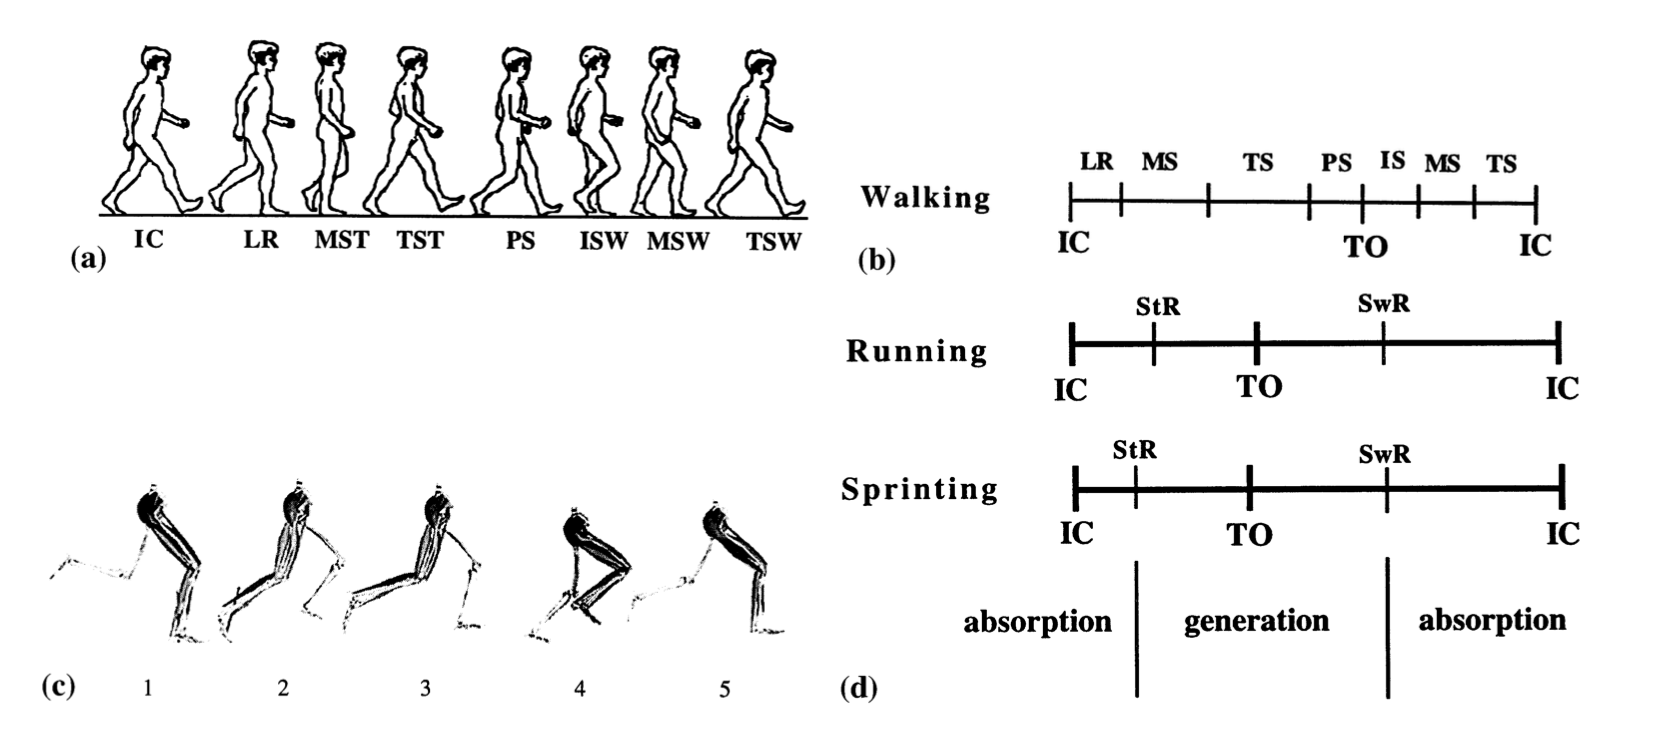
\includegraphics[width=1\textwidth]{Images/The gait cycle running walking}
	\caption{The gait cycle. a. Walking figure. b. Walking gait cycle: *IC, initial contact; LR, loading response; *TO, toe off; MS, midstance; TS, terminal stance; PS, preswing; IS, initial swing; MS, midswing; TS, terminal swing. c. Running figure: 1. Stance phase absorption. 2. Stance phase generation. 3. Swing phase generation. 4. Swing phase reversal. 5. Swing phase absorption. *Musculoskeletal animation produced using SIMM (Software for Musculoskeletal Modelling, Musculographics, Chicago, Illinois). d. Running gait cycle: *for running and sprinting; IC, initial contact; TO, toe off; StR, stance phase reversal; SwR, swing phase reversal; absorption, from SwR through IC to StR; generation, from StR through TO to SwR. }
	\label{Images/The gait cycle running walking}
\end{figure}



Running is a fast and vigorous form of movement, and is characterized by the absence of periods when both feet are in contact with the ground and by the presence of two periods of double float, one at the beginning and one at the end of the swing phase. The timing of toe off occurs before 50\% of the gait cycle is completed and is faster in running. Additionally, running is characterized by alternate periods of acceleration and deceleration known as absorption and generation, which do not coincide with the timing of initial contact and toe off \autoref{Images/The gait cycle running walking}. These characteristics are also affected by the speed of the runner, faster runners have less time in stance and toe off earlier in the gait cycle.
During running, the foot typically strikes the ground with the heel and then quickly rolls forward to push off with the toe, it has a greater stride length compared to Walking, and a segnificant thigh angle. \cite{Novacheck:1998} 

 \begin{figure}
 	\centering
 	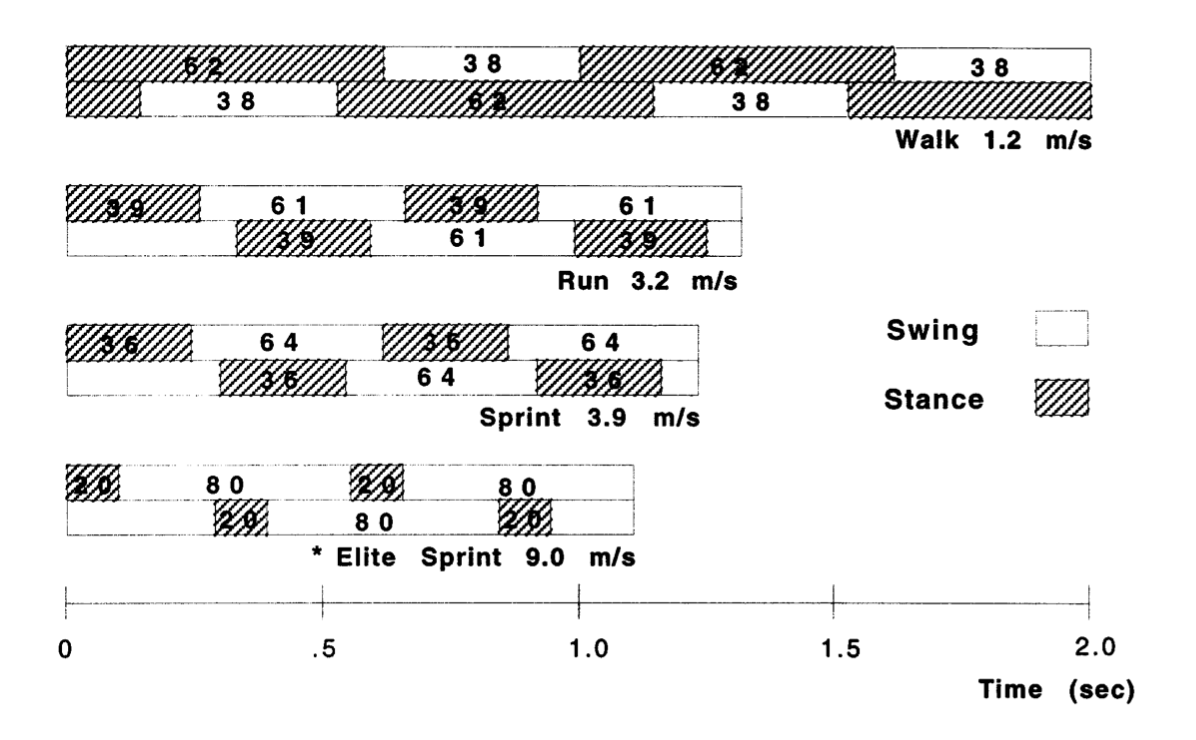
\includegraphics[width=1\textwidth]{Images/Variation in gait cycle parameters with speed of movement.}
 	\caption{Variation in gait cycle parameters with speed of movement. For each condition, the bar graph begins at initial contact on the left and represents two complete gait cycles or strides. Note that as speed increases, time spent in swing (clear) increases, stance time (shaded) decreases, double float increases, and cycle time shortens. Informa- tion for this graph comes from data collected at the Motion Analysis Lab at Gillette Children’s Specialty Healthcare. *Data for elite sprinting is from Vaughan [16]. \cite{Novacheck:1998} }
 	\label{Images/Variation in gait cycle parameters with speed of movement.}
 \end{figure}

Jumping is a sudden, explosive movement where both feet leave the ground at the same time and is most commonly used for vertical displacement, the thigh angle is . Jumping is a complex and highly coordinated movement, which can be performed in many ways such as for example for athletic events like high jump, long jump or pole vault. 

The use of an Inertial Measurement Unit (IMU) is an effective method for measuring the unique characteristics of walking, running, and jumping. IMUs are advantageous in this context as they are portable, energy-efficient, cost-effective, durable, and reliable. This makes them ideal for measuring the various events associated with these forms of human locomotion. \cite{ThiThuVu:2020}. 

Standard IMUs measure the rotational velocity around three axis using gyroscopes, linear accelerations, and the strength of the magnetic field along those same axes, utilizing accelerometers and magnetometers.: running and walking are distinguished by speed and thigh angle, while jumping is characterized by the direction of movement.

In walking, the thigh angle typically decreases during the stance phase and increases during the swing phase, while in running, the thigh angle typically increases during the stance phase and decreases during the swing phase. Jumping involves a larger thigh angle excursion than both walking and running.

Additionally, the accelerometer present on our board  also helps detect and classify walking, running, and jumping. The study conducted in \cite{Kwapisz:2010}  have proven that accelerometer data can be enough for diffrent classification techniques to accuratly distinguish the type of motion. more detail about this will be in chapter 7 Datasets. 


However, it is important to note that while the thigh angle can provide some information about a person's gait pattern, it is not the only factor that needs to be considered. Other factors such as the foot trajectory, ankle angle and the knee angle also play an important role in identifying walking, running and jumping. Also, It is also important to consider that this is a very complex process and there is much research ongoing to improve the accuracy of gait detection and classification. Furthermore, there are many factors that can influence the thigh angle such as shoes, surfaces, and age among others.


%https://slideplayer.com/slide/12956873/


